\documentclass{beamer}
\usetheme{Madrid}
\usepackage{polski}

\usepackage{amsmath}
\usepackage{listings}

\title{Symulacja ruchu ciał niebieskich}
\author{Wiktor Przadka}
\date{Listopad 2020}

\begin{document}

\maketitle

\section{Model}

\begin{frame}{Wstęp}
    \begin{block}{Opis Problemu}
        Problem n-ciał polega na przewidywaniu toru ruchu planet w przestrzeni kosmicznej. Rozwiązanie problemu można sprowadzić do rozwiązania układu równań różniczkowych zwyczajnych.
    \end{block}
    \begin{block}{Motywacja}
        Motywacją problemu jest chęć zrozumienia ruchu skomplikowanych formacji ciał, takich jak galaktyki i możliwość przewidzenia pozycji ciał niebieskich w czasie.
    \end{block}
    \begin{block}{Rozwiązanie}
        Obecnie rozwiązanie analityczne jest znane jedynie dla problemu 2-ciał. dla większej ilości ciał nie znamy żadnych analitycznych metod rozwiązania układu równań opisujących ruch ciał. Z tego powodu musimy używać rozwiązań numerycznych.
    \end{block}
\end{frame}

\begin{frame}{Model matematyczny}
    \begin{block}{Układ równań grawitacyjnych Newtona}
        Siły między ciałami o indeksach k i j opisywane są wzorami:
        $$ F_{k,j} = G \frac{ m_{k} m_{j} }{ \| x_{k} - x_{j} \|^2 }\ \forall_{k, j \in n} $$
        $$ \vec{F_{k,j}} 
        = G \frac{ m_{k} m_{j} }{ \| x_{k} - x_{j} \|^2 } 
        \Big( \frac{ x_{k} - x_{j} }{\| x_{k} - x_{j} \|} \Big) 
        = G \frac{ m_{k} m_{j} }{ \| x_{k} - x_{j} \|^3 }(x_{k} - x_{j})\ \forall_{k, j \in n} $$
        Gdzie:\\
        G = $6.6743\cdot 10^{-11} [\frac{m^3}{kg \cdot s^2}]$ - stała grawitacyjna \\
        $m_{i}$ - masa i-tego ciała [kg]\\
        $x_{i}$ - pozycja i-tego ciała w przestrzeni\\
        $\| x_{i} - x_{j} \|$ - odległość między ciałami i,j [m]\\
    \end{block}
\end{frame}

\begin{frame}{Model matematyczny}
    \begin{block}{Układ równań różniczkowych zwyczajnych}
        Siła dla ciała o indeksie k opisana jest wzorem:
        $$ F_{k} 
        = m_{k} a_{k} 
        = m_{k} \frac{\partial v}{\partial t} 
        = m_{k} \frac{\partial^2 x}{\partial t^2} $$
        stąd dostajemy:
        $$ \vec{F_{k}}
        = \sum_{j = 0}^{n} G \frac{ m_{k} m_{j} }{ \| x_{k} - x_{j} \|^3 }(x_{k} - x_{j})$$
        
        $$ m_{k} \frac{\partial^2 x_{k}}{\partial t^2}
        = G\cdot \sum_{j = 0}^{n} \frac{ m_{k} m_{j} }{ \| x_{k} - x_{j} \|^3 }(x_{k} - x_{j})$$
        
        $$ \frac{\partial^2 x_{k}}{\partial t^2}
        = G\cdot \sum_{j = 0}^{n} \frac{ m_{j} }{ \| x_{k} - x_{j} \|^3 }(x_{k} - x_{j})$$
    \end{block}
\end{frame}

\begin{frame}{Model matematyczny}
    \begin{block}{Model w postaci zmiennych stanu}
        (1) $$ \frac{\partial x_{k}}{\partial t} = v_{k}$$
    
        (2) $$ \frac{\partial v_{k}}{\partial t}
        = G\cdot \sum_{j = 0}^{n} 
        \frac{ m_{j} }{ \| x_{k} - x_{j} \|^3 }
        (x_{k} - x_{j})$$
    \end{block}
    \begin{block}{(*)}
        Jest to model, użyty w symulacji przedstawionej w kolejnej sekcji    
    \end{block}
\end{frame}

\section{Symulacja}

\begin{frame}{Symulacja}
    \begin{block}{Symulacja}
        Symulacja została napisana w języku C++ przy użyciu bioblioteki graficznej SFML, kod dostępny jest w repozytorium na github'ie pod linkiem:\\
        \href{https://github.com/wprzadka/modeling_and_simulation/tree/main/n-body-problem}
        {https://github.com/wprzadka/modeling\_and\_simulation/tree/main/\\n-body-problem}
    \end{block}
    \begin{block}{Dodatkowe założenia}
        Symulacja wyliczana jest na 2 wymiarowej płaszczyźnie, z tego powodu bliskie spotkania między ciałami niebieskimi nie są traktowane jako kolizje. Symulacja traktuje je raczej jako mijanie się ciał w 3 wymiarze przestrzennym.
    \end{block}
\end{frame}

\begin{frame}{Symulacja}
    \begin{block}{Ruch pięciu ciał o jednakowych masach}
        \begin{center}
            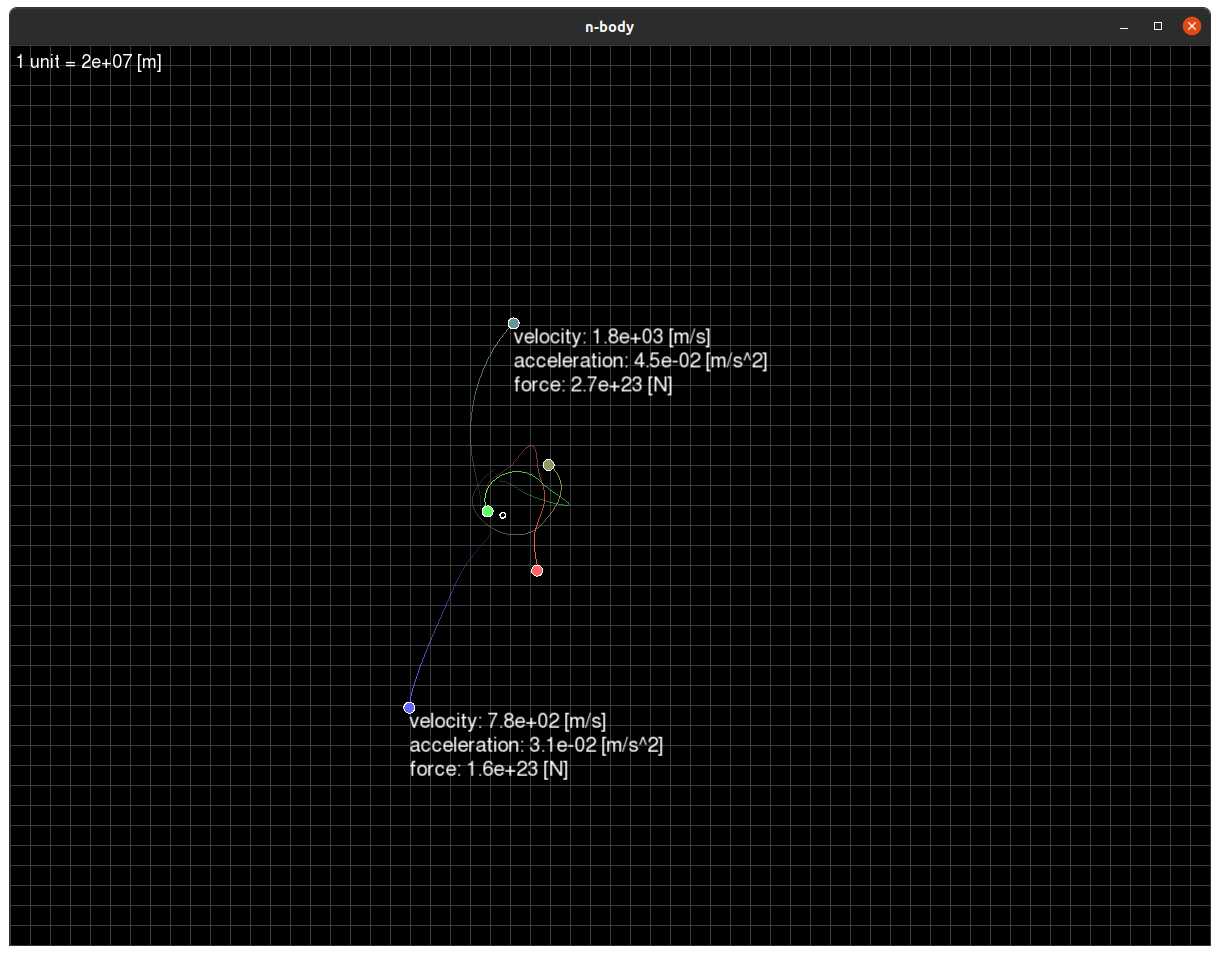
\includegraphics[width=8cm]{./img/five-bodies.png}
        \end{center}
    \end{block}
\end{frame}

\begin{frame}{Symulacja}
    \begin{block}{System słoneczny}
        \begin{center}
            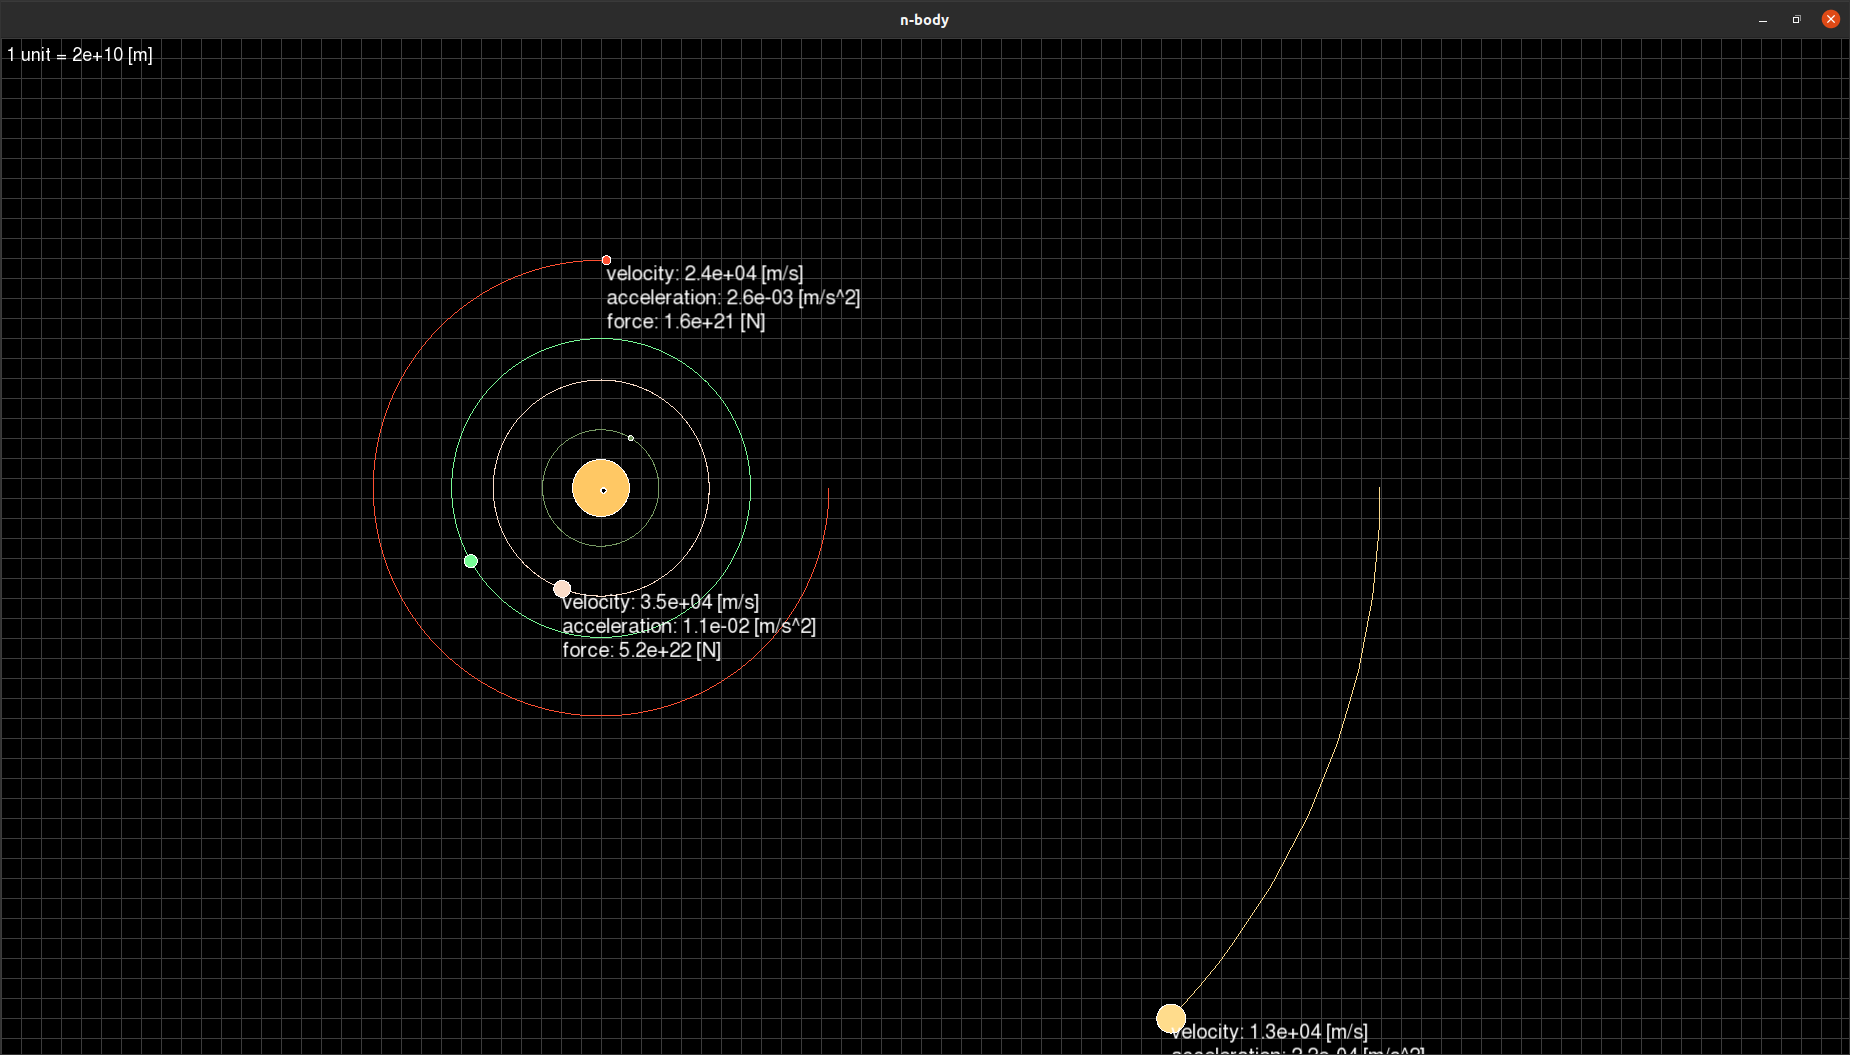
\includegraphics[width=8cm]{./img/solar-system.png}
        \end{center}
    \end{block}
\end{frame}

\begin{frame}{Symulacja}
    \begin{block}{Precyzja obliczeń}
        Wszelkie obliczenia oraz stałe wykorzystywane w symulacji są zapisane w zmiennych o dużej precyzji - long double
    \end{block}
    \begin{block}{Niedokładności symulacji}
        Wszelkie niedokładności w symulacji wynikają z ograniczonej precyzji zmiennych wykorzystywanych do obliczeń oraz niedokładności metody Eulera wykorzystywanej do rozwiązywania układu równań różniczkowych zwyczajnych.
    \end{block}
\end{frame}

\section{walidacja}

\begin{frame}{Walidacja}
    \begin{block}{Środek masy systemu}
        Z zasady zachowania momentu pędu wynika, że środek masy systemu izolowanego od zewnętrznych sił może poruszać się jedynie ze stałą prędkością. Oznacza to, że jeśli w chwili rozpoczęcia symulacji $t_{0}$ ciała są w spoczynku to w każdym momencie czasu symulacji $t_{i}$ koordynaty środka ciężkości systemu muszą być położone w jednym punkcie.
    \end{block}
\end{frame}

\begin{frame}{Walidacja}
    \begin{block}{Środek masy układu trzech ciał}
        \begin{center}
            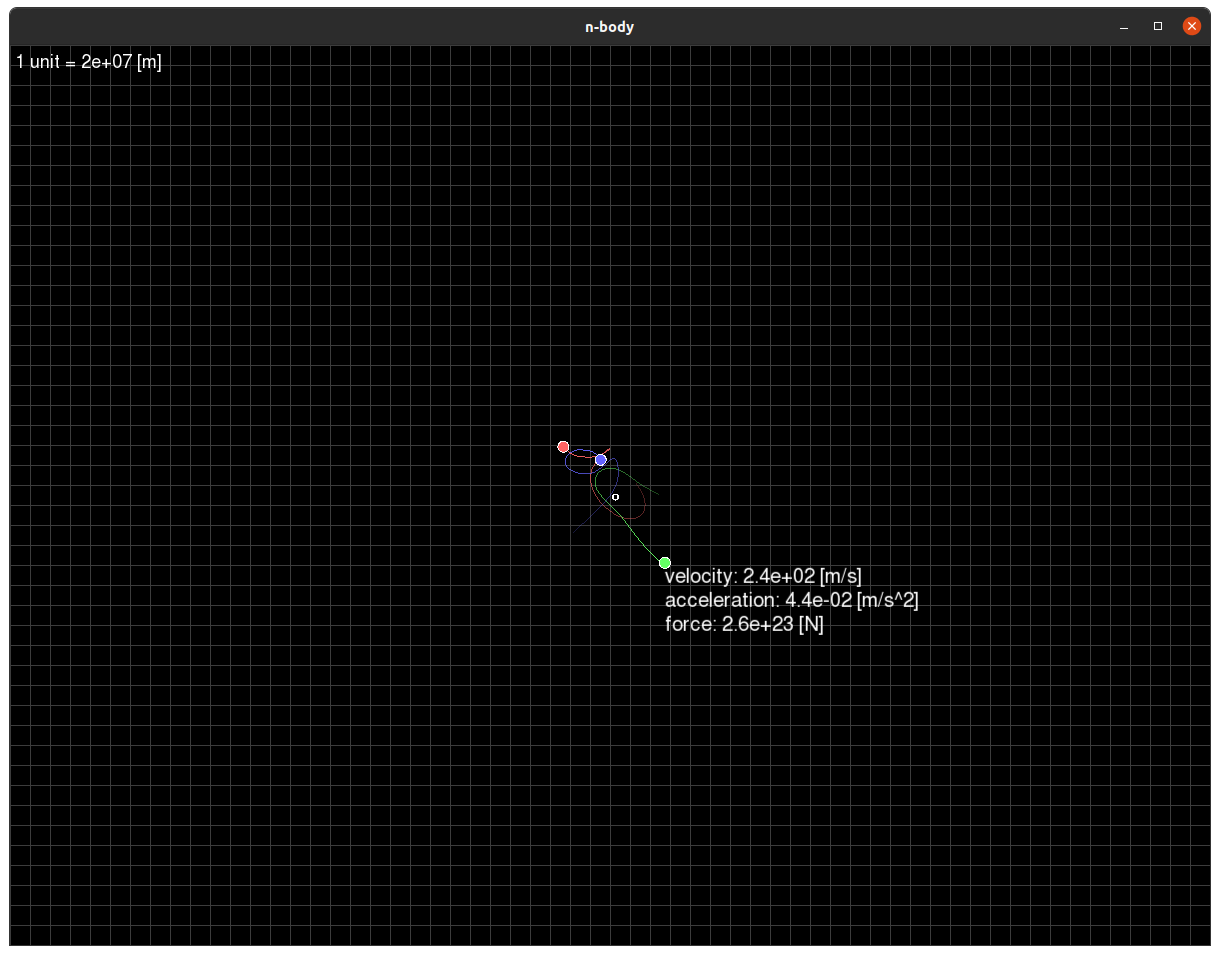
\includegraphics[width=8cm]{./img/three-bodies.png}
        \end{center}
    \end{block}
\end{frame}

\begin{frame}{Walidacja}
    \begin{block}{Siła między Ziemią a Słońcem}
        $F_{z,s} = G\cdot \frac{m_{z}\cdot m_{s}}{(r_{s,z})^2} = \\
        = 6.6743\cdot 10^{-11}\cdot 
        \frac{5.972\cdot 10^{24}\cdot 1.989\cdot 10^{30}}
        {(1.496 * 10^{11})^2} = 3.5423961\cdot 10^{22}\ [N]$
    \end{block}
    
    \begin{block}{Ruch Ziemi wokół Słońca}
        Dystans między środkami masy ziemi i słońca wynosi\\ 
        $r_{s,z} = 1.496e11\ [m]$.\\
        Ziemia pokonuje więc\\ 
        $d_z = 2 \pi \cdot 1.496\cdot 10^{11} [m] = 9.39488\cdot 10^{11} [m]$\\
        w czasie\\ 
        $T_z = 365.25 [dni] = 365.25\cdot 24\cdot 60\cdot 60 [s] = 3.15576\cdot 10^{7} [s]$.\\
        Co daje średnią szybkość ruchu ziemi równą\\
        $v_z = d_z / T_z 
        = \frac{9.39488\cdot 10^{11}}{3.15576\cdot 10^{7}} 
        = 2.97705782442\cdot 10^{4} [\frac{m}{s}]$
    \end{block}
\end{frame}

\begin{frame}{Walidacja}
    \begin{block}{Słońce - Ziemia}
        \begin{center}
            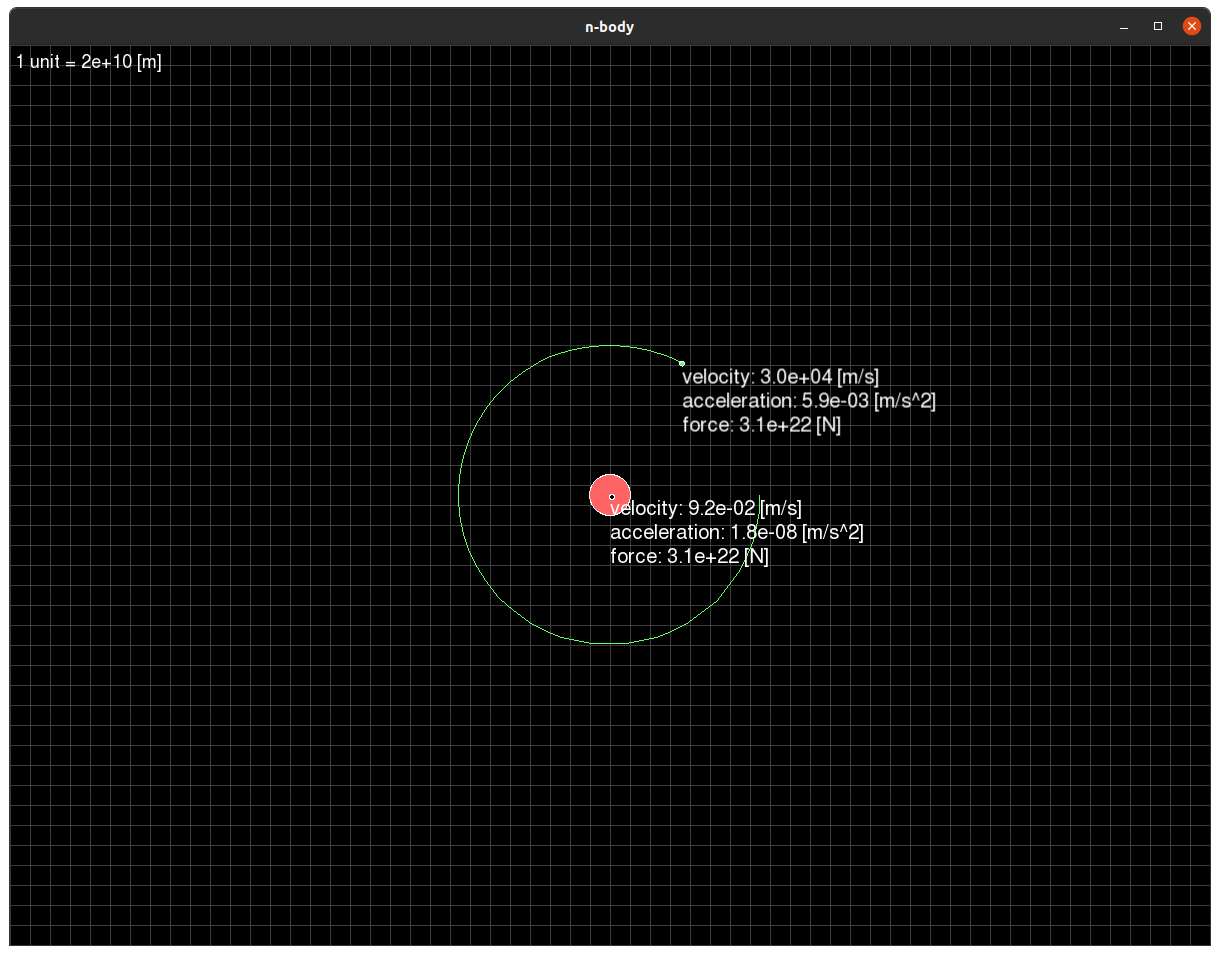
\includegraphics[width=8cm]{./img/sun-earth.png}
        \end{center}
    \end{block}
\end{frame}

\begin{frame}{Walidacja}
    \begin{block}{Siła między Ziemią a Księżycem}
        $F_{z,k} = G\cdot \frac{m_{z}\cdot m_{k}}{(r_{z,k})^2} = \\
        = 6.6743\cdot 10^{-11}\cdot 
        \frac{5.972\cdot 10^{24}\cdot 7.34767309\cdot 10^{22}}
        {(3.844 * 10^{8})^2} = 1.9820225\cdot 10^{20}\ [N]$
    \end{block}
    
    \begin{block}{Ruch Księżyca wokół Ziemi}
        Dystans między środkami masy ziemi i słońca wynosi\\ 
        $r_{z,k} = 384.4e6\ [m]$.\\
        Ziemia pokonuje więc\\ 
        $d_k = 2 \pi \cdot 384.4\cdot 10^{6} [m] = 2.41525643208\cdot 10^{9} [m]$\\
        w czasie\\ 
        $T_k = 27.3 [dni] = 27.3\cdot 24\cdot 60\cdot 60 [s] = 2.358720\cdot 10^{6} [s]$.\\
        Co daje średnią szybkość ruchu księżyca równą\\
        $v_k = d_k / T_k 
        = \frac{2.41525643208\cdot 10^{9}}{2.358720\cdot 10^{6}} 
        = 1.02396911549\cdot 10^{3} [\frac{m}{s}]$
    \end{block}
\end{frame}

\begin{frame}{Walidacja}
    \begin{block}{Ziemia - Księżyc}
        \begin{center}
            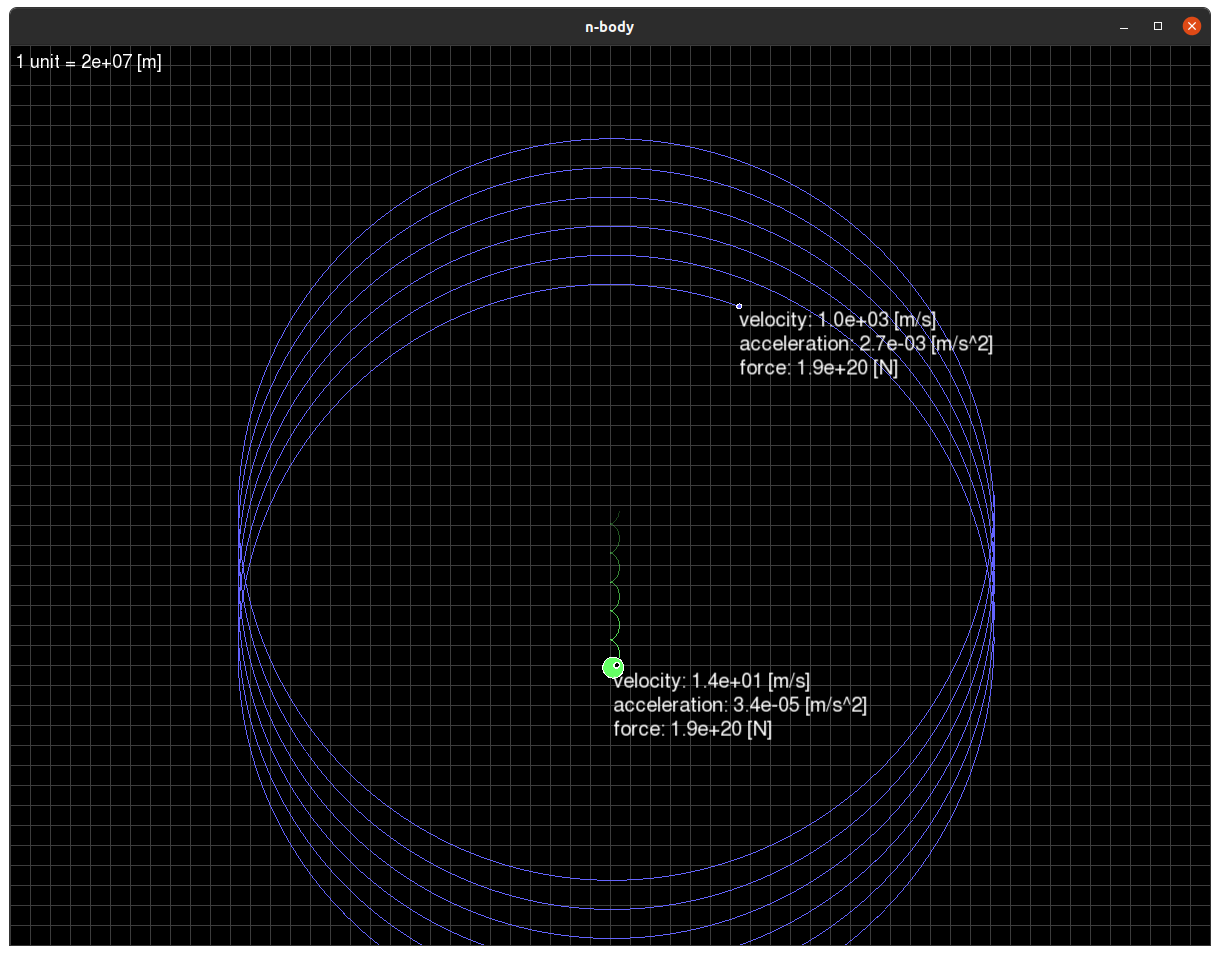
\includegraphics[width=8cm]{./img/earth-moon.png}
        \end{center}
    \end{block}
\end{frame}

\end{document}
